\documentclass{standalone}

\usepackage{tikz}
\usetikzlibrary{calc}

\begin{document}
  %noformat{
  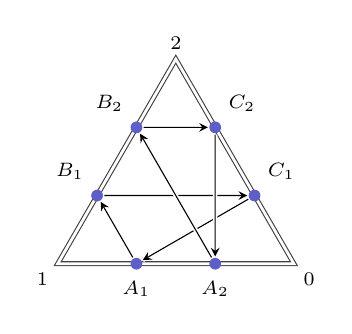
\begin{tikzpicture}
    \tikzstyle{v1} = [circle, outer sep=0.5pt, fill, inner sep=1.5pt]
    \tikzstyle{v2} = [circle, outer sep=0.5pt, fill, inner sep=3.0pt]
    \tikzstyle{unf} = [color=darkgray]
    \tikzstyle{frz} = [color=blue!60!darkgray!70]
    \tikzstyle{r} = [color=red!70!darkgray!70]
    \tikzstyle{e} = [->, >={stealth}, preaction={draw=white, -, ultra thick}]
    \tikzstyle{b} = [fill, fill opacity=0.0, circle, outer sep=0.5pt, inner sep=1.5pt]
    \tikzstyle{te} = [color=darkgray, double distance=1pt]
    \tikzstyle{h} = [dashed, color=gray, ->, >={stealth}]

    \tikzset{font=\scriptsize}

    \begin{scope}
      \coordinate[label={330:$0$}] (l_0) at (-30:1.7321);
      \coordinate[label={210:$1$}] (l_1) at (210:1.7321);
      \coordinate[label={ 90:$2$}] (l_2) at ( 90:1.7321);

      \draw[te] (l_0) -- (l_1) -- (l_2) -- cycle;

      \node[v1, frz, label={120:$B_1$}   ] (B1)  at ($ (l_1) + ( 60:1.0)$) {};
      \node[v1, frz, label={120:$B_2$}   ] (B2)  at ($ (l_1) + ( 60:2.0)$) {};
      \node[v1, frz, label={270:$A_2$}   ] (A2)  at ($ (l_1) + (  0:2.0)$) {};
      \node[v1, frz, label={270:$A_1$}   ] (A1)  at ($ (l_1) + (  0:1.0)$) {};
      \node[v1, frz, label={ 60:$C_1$}   ] (C1)  at ($ (l_2) + (-60:2.0)$) {};
      \node[v1, frz, label={ 60:$C_2$}   ] (C2)  at ($ (l_2) + (-60:1.0)$) {};

      \draw[e] ( C1) -- ( A1);
      \draw[e] ( A1) -- ( B1);
      \draw[e] ( B1) -- ( C1);

      \draw[e] ( C2) -- ( A2);
      \draw[e] ( A2) -- ( B2);
      \draw[e] ( B2) -- ( C2);
    \end{scope}
  \end{tikzpicture}
  %}noformat
\end{document}
